% !TeX root = ../presentation.tex

\section{Results}
\begin{frame}{Nearest Neighbor Interpolation}
	\centering
	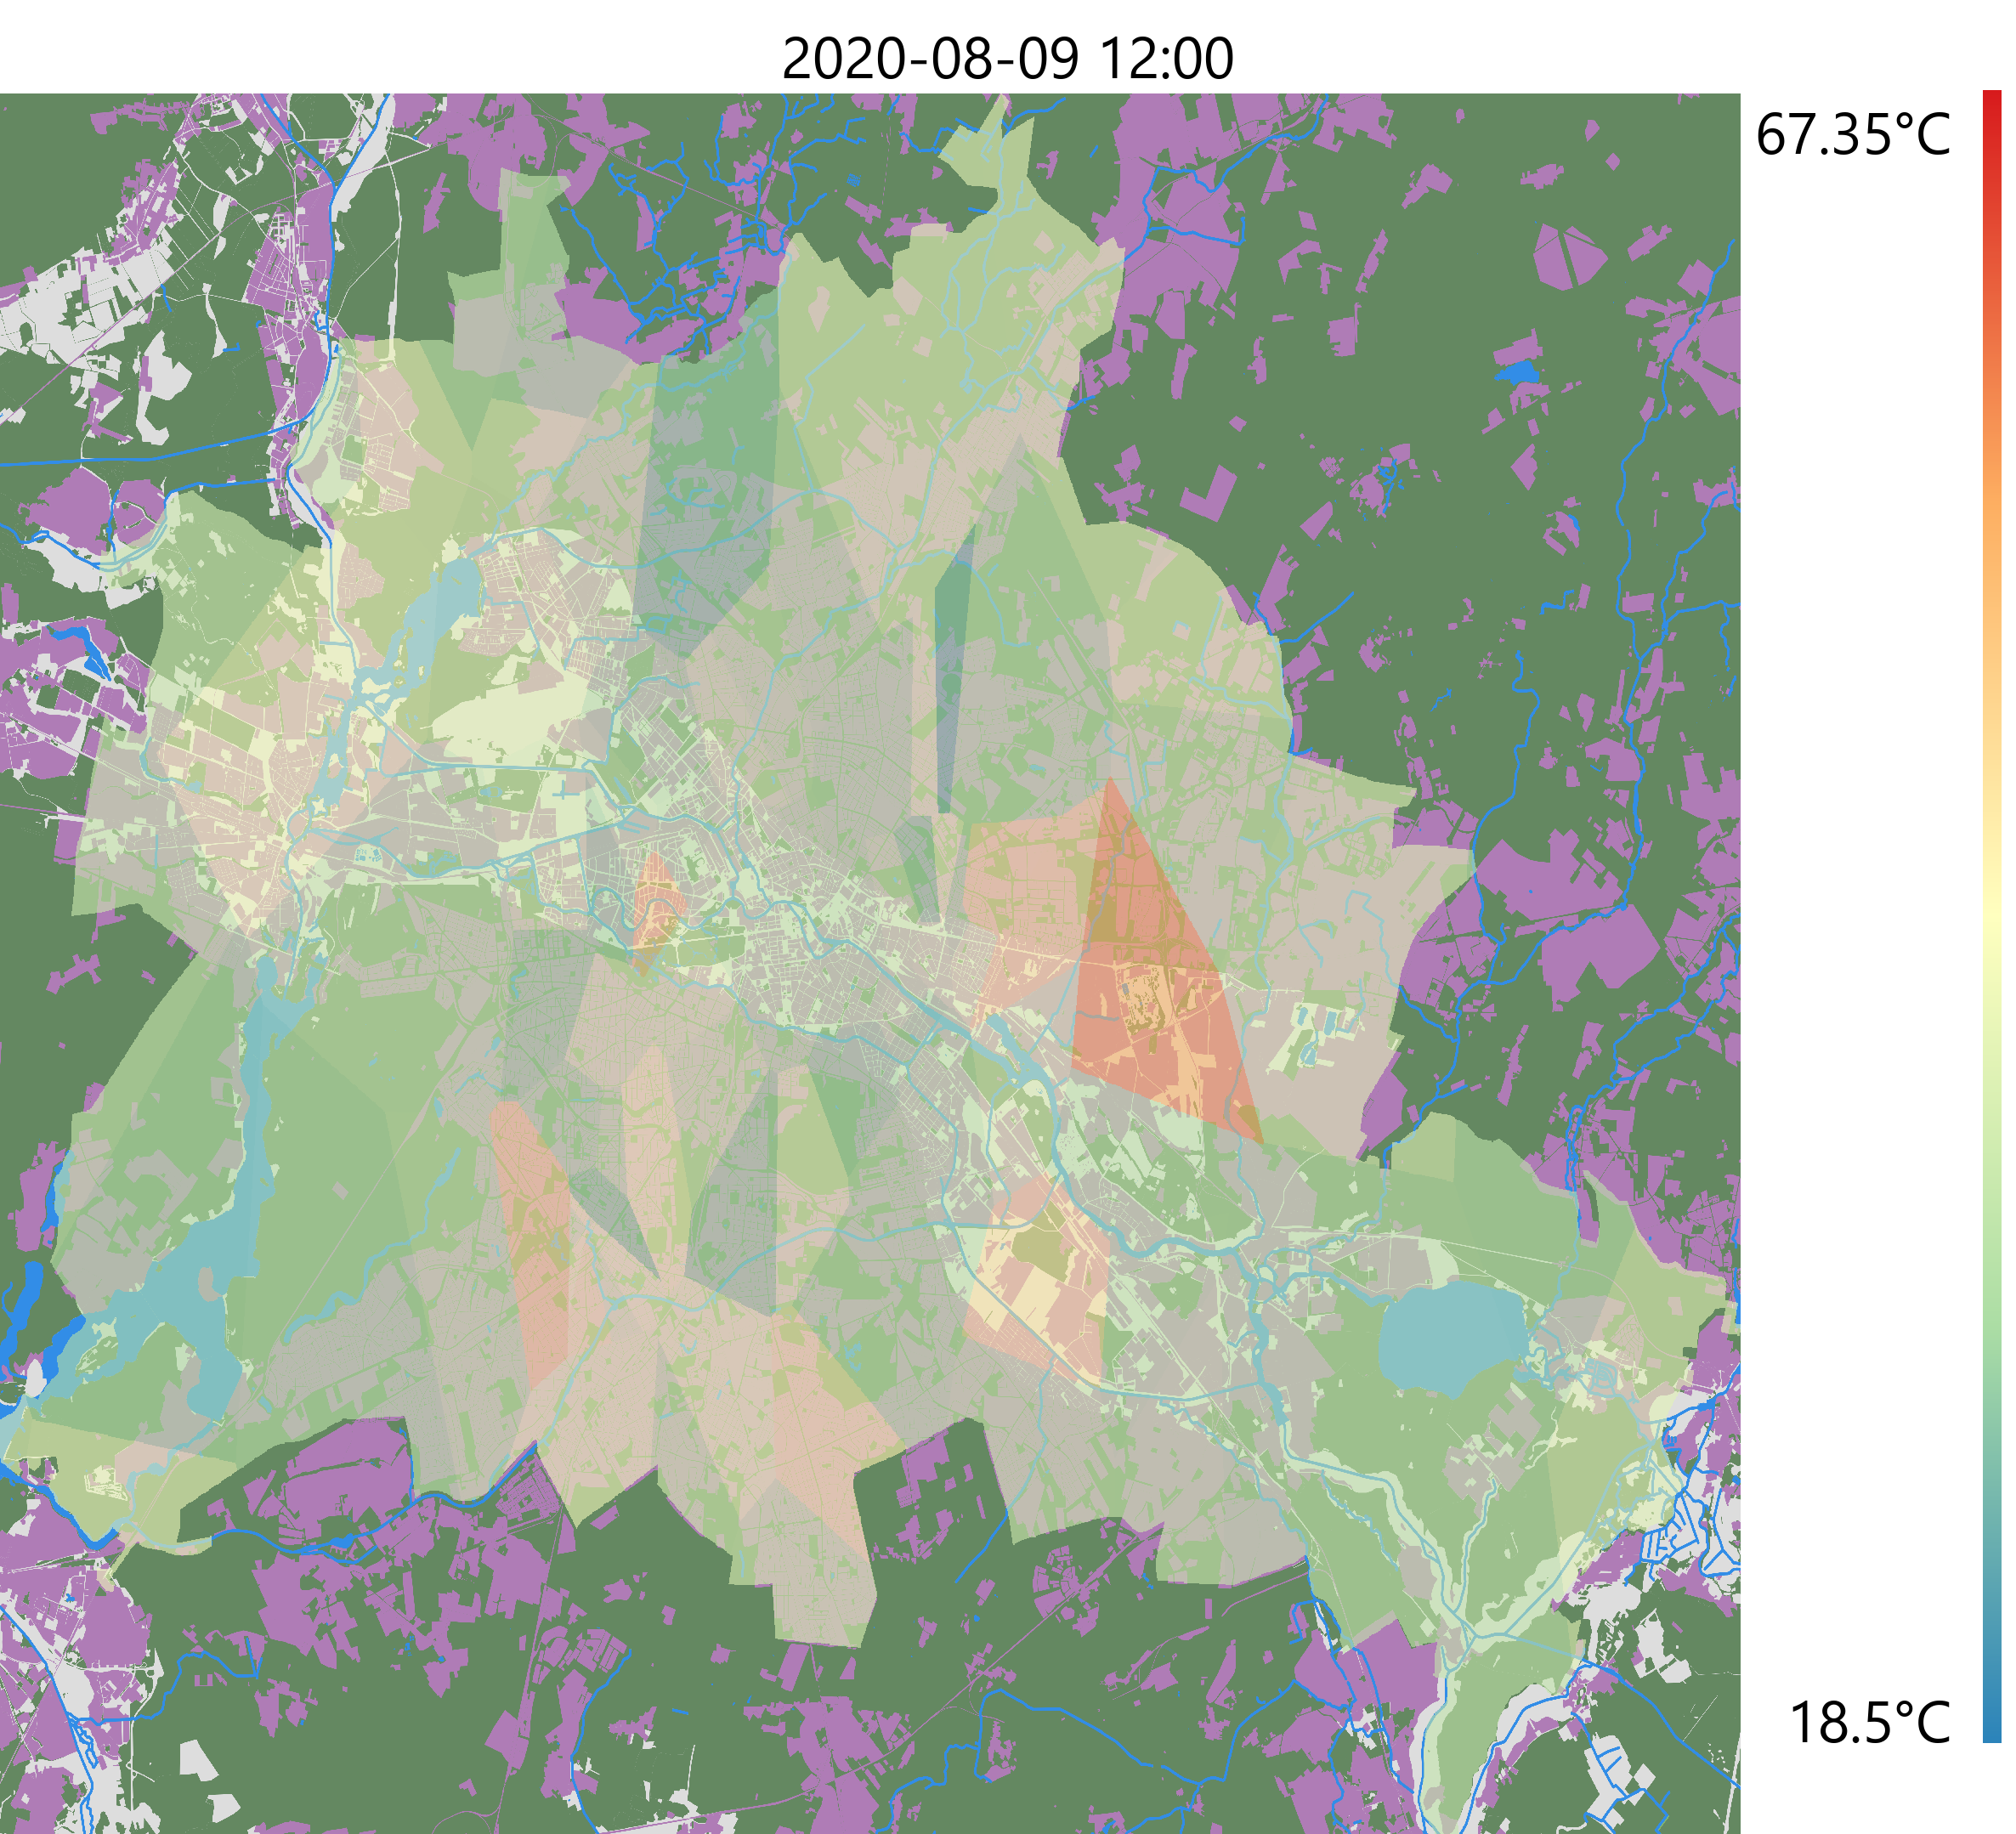
\includegraphics[height=\textheight,keepaspectratio]{../writeup/images/hot_2020-08-09_12_00_nearest.png}
\end{frame}
\begin{frame}{TIN Interpolation}
	\centering
	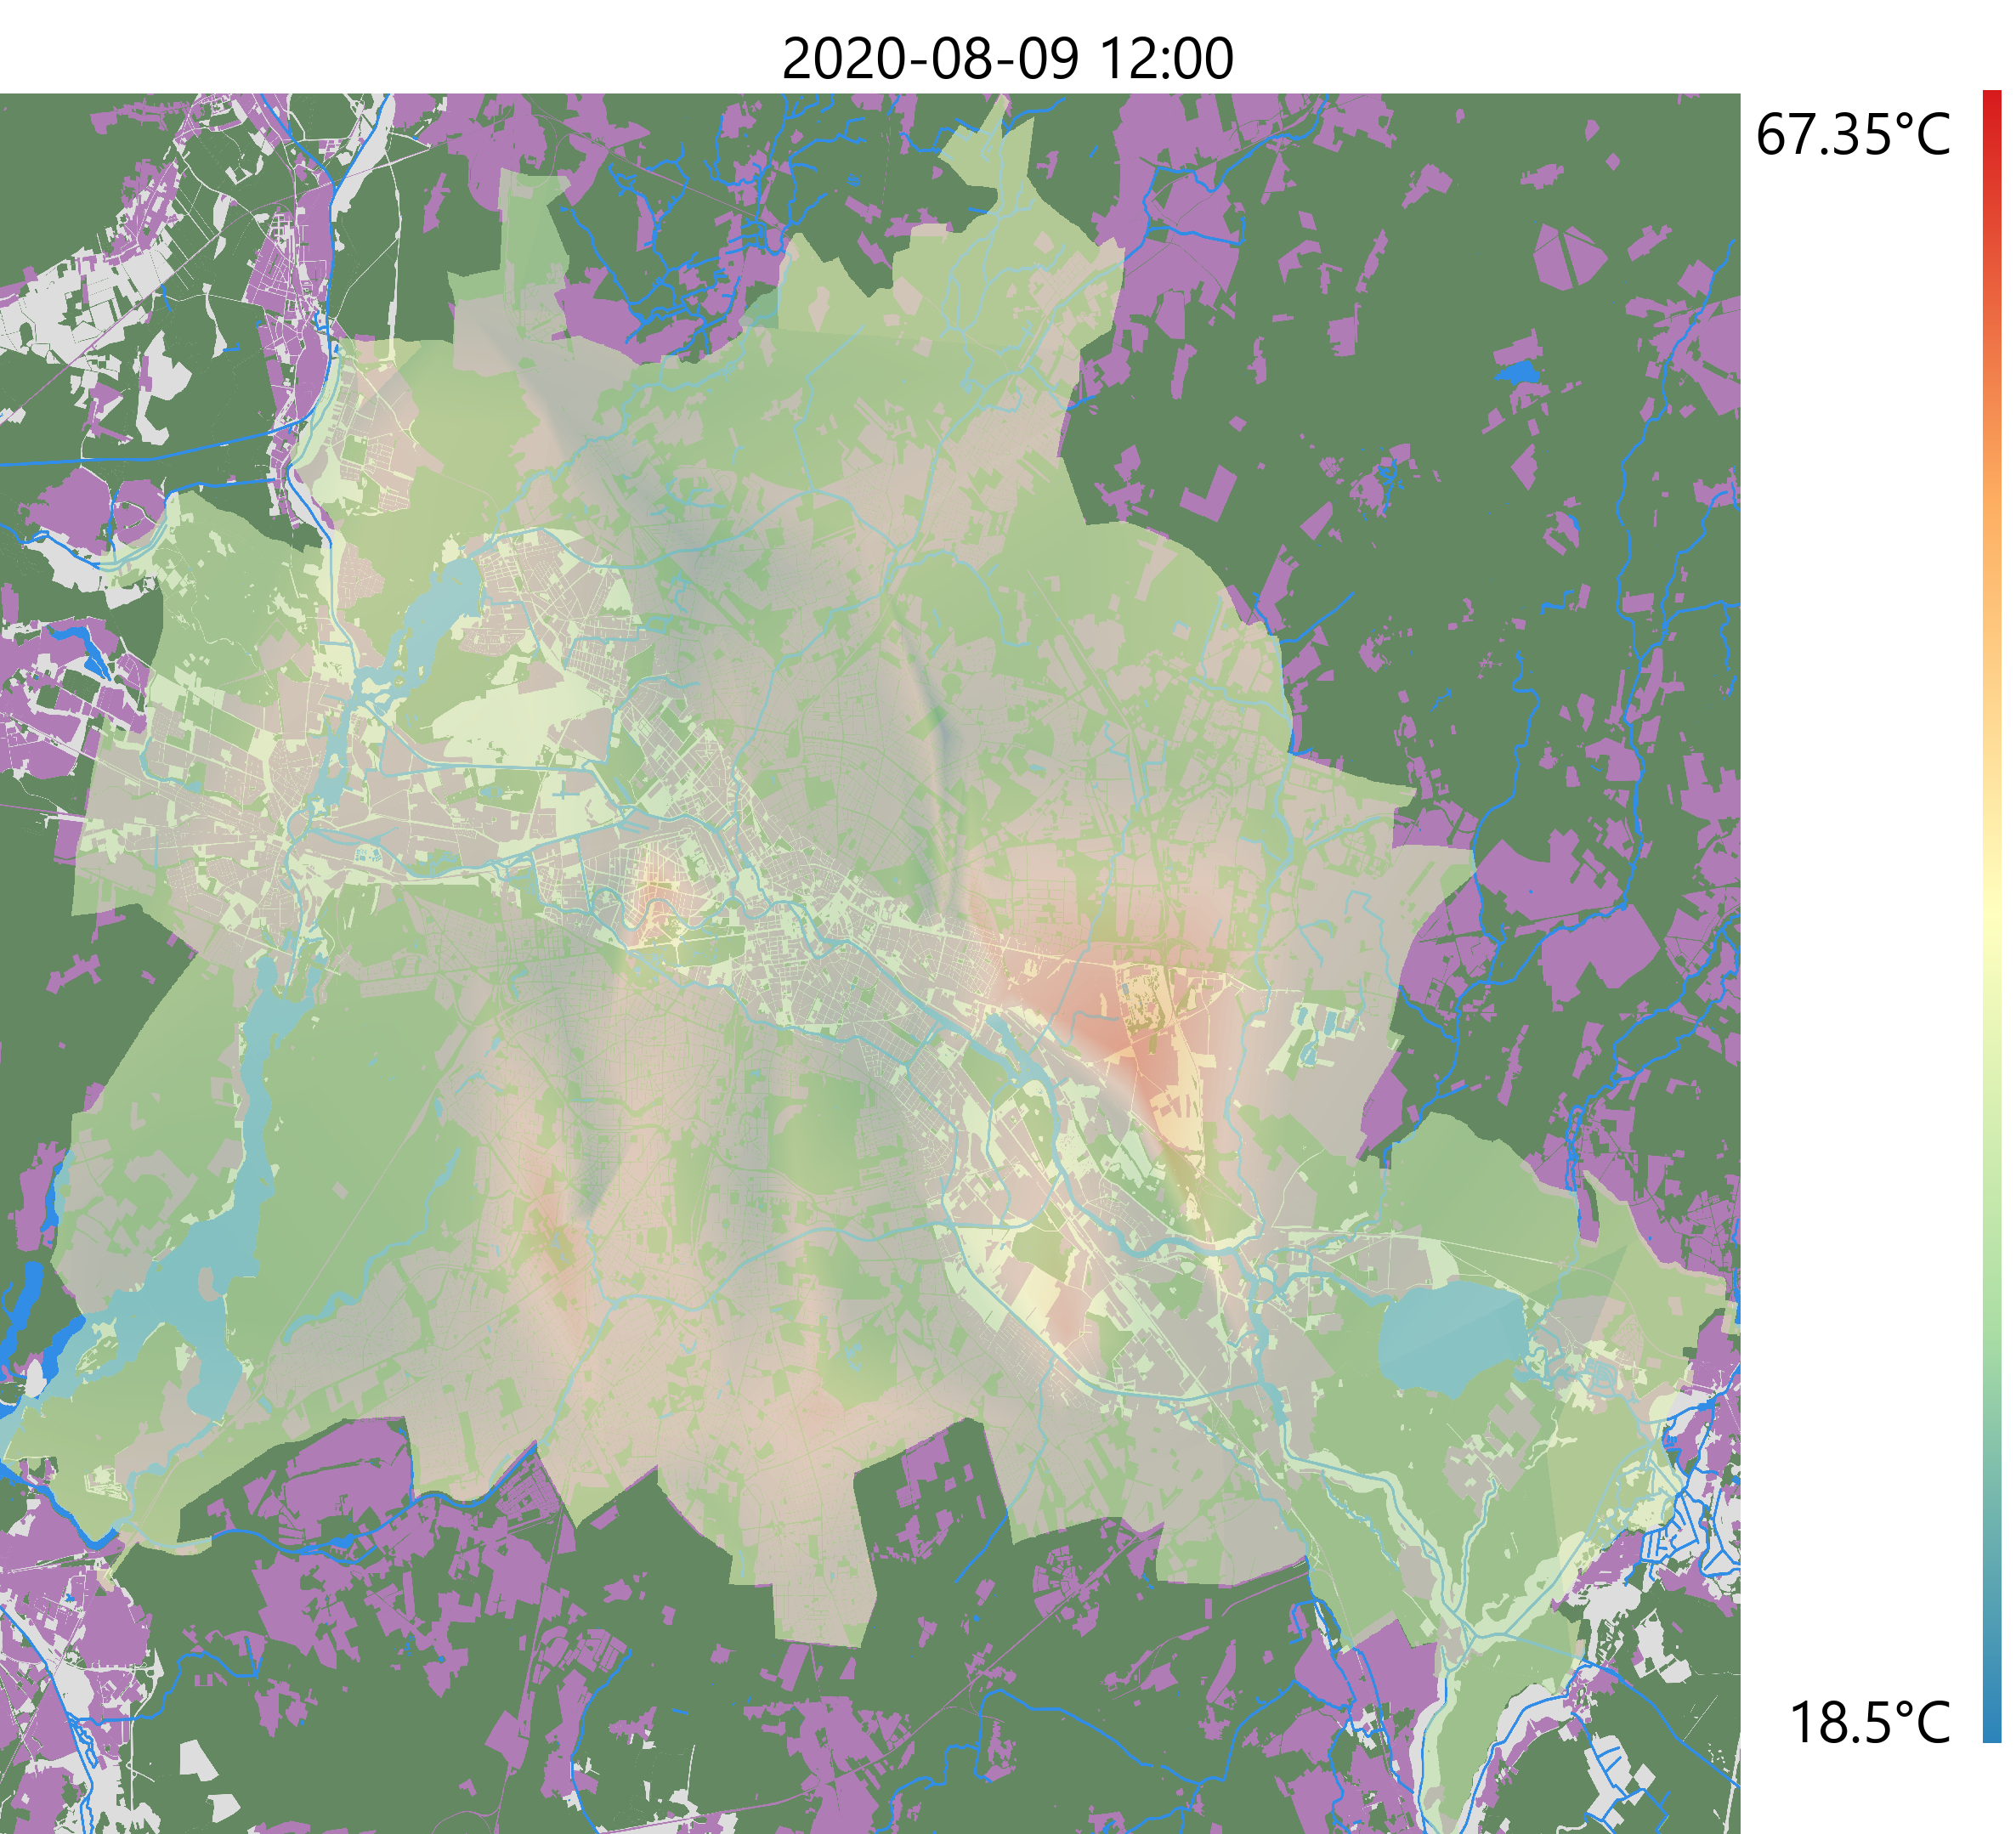
\includegraphics[height=\textheight,keepaspectratio]{../writeup/images/hot_2020-08-09_12_00_linear.png}
\end{frame}
\begin{frame}{IDW Interpolation}
	\centering
	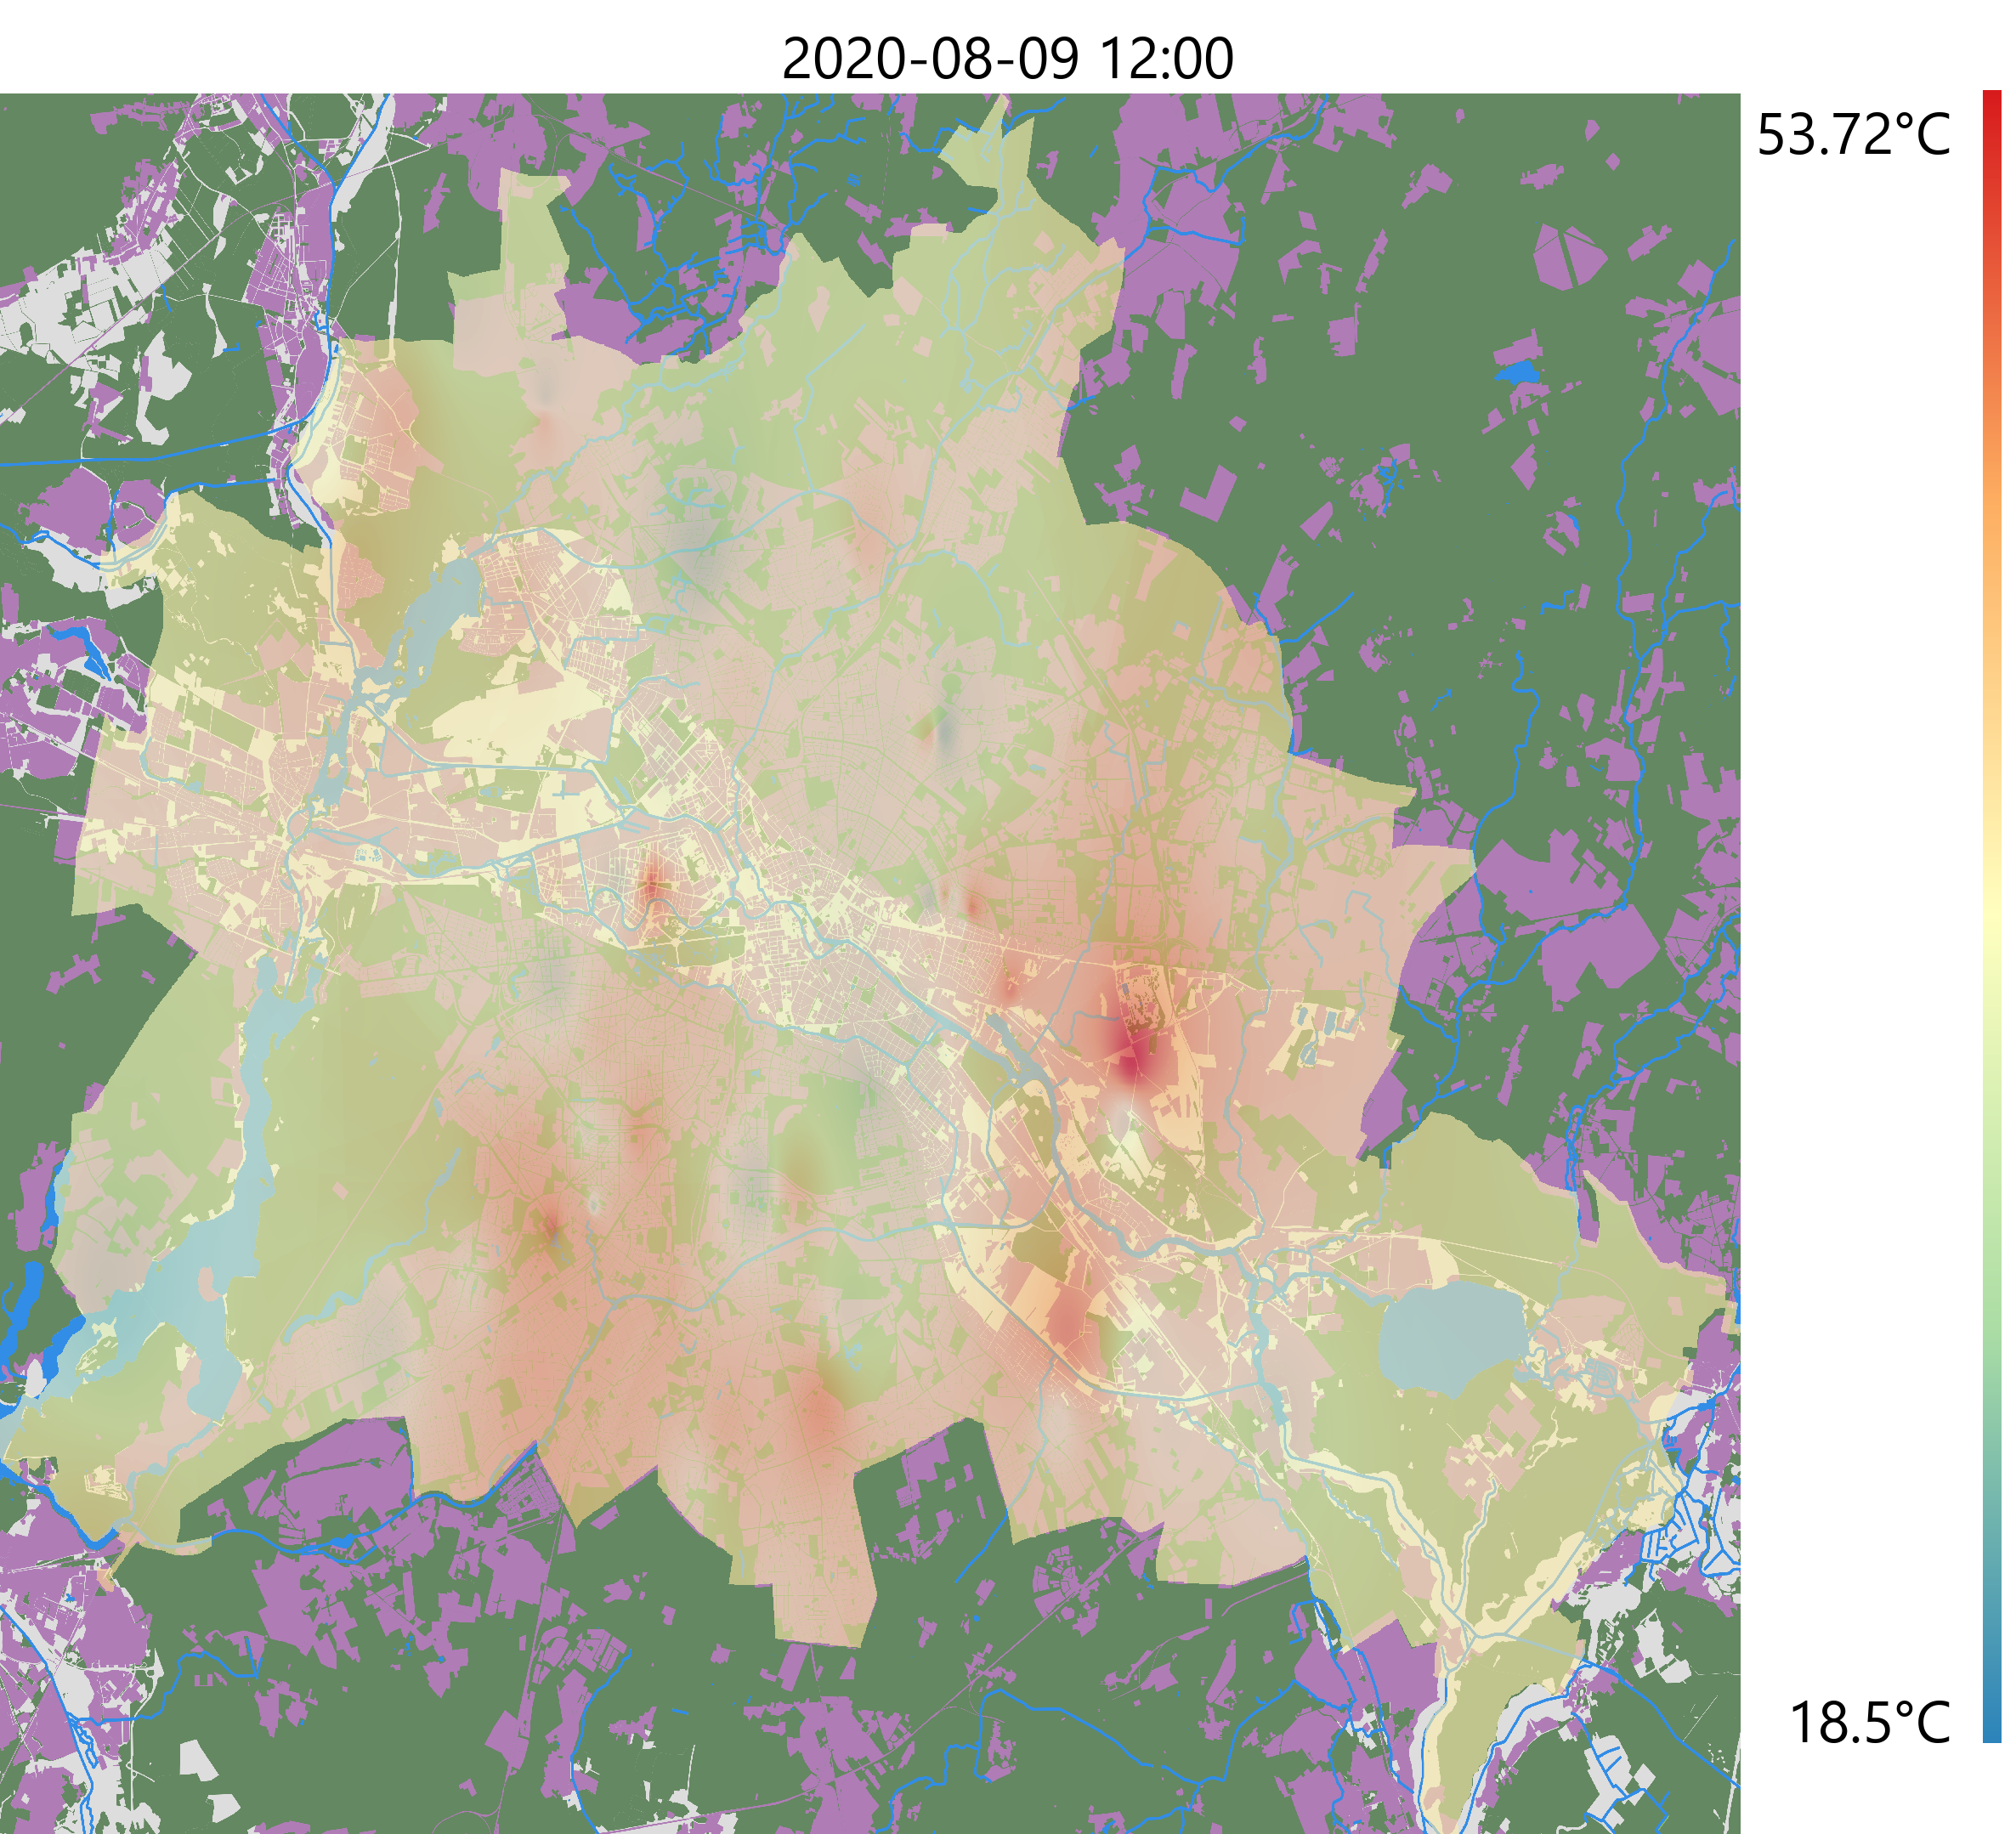
\includegraphics[height=\textheight,keepaspectratio]{../writeup/images/hot_2020-08-09_12_00_invdistnn.png}
\end{frame}
\begin{frame}{Discussion}
	\begin{itemize}
		\item Why did we choose GDAL?
		\item Why did we choose Nearest Neighbor, TIN and IDW?
	\end{itemize}
\end{frame}